\abstract{To Be Done}

\chapter*{Introduction}
The increasing number of sensors and intelligence in most of our equipment has launched a new era. In order to kill the HIPPO\footnote{Highest Paid Person's Opinion}, our society is now heavily relying on data-driven decision. 

This shift was initiated by the spectacular increase in data collection. The amount of data to be analyzed has became prohibitively high. That is the case of UPC Cablecom. The company has started to accumulate a lot of data: tracking the health of their equipment and most importantly of CPEs\footnote{Customer premises equipment (e.g. set top box, router, ...)}. 

The scope of this project is to leverage this data to improve customer's experience. Combining customer feedback to CPE's health indicators, the goal is to predict failure of such equipment and increase customer's retention.

The telecommunication company tracks every interaction between customer care and their customer which can be used in order to detect CPEs that are experiencing problems. Nevertheless the project consisted in multiple challenges that shall be discussed in the following pages:
\begin{itemize}
    \item While we can identify failing CPEs using data created by customer care, on the remaining CPEs we cannot be sure to be in the presence of a healthy equipment as it could simply be the case that the customer hasn't reached customer care (yet). 
    \item The data that can be used comes from different sources and a proper matching needs to be done. Some databases proved to be unusable and the help of experts was often necessary in order to determine a good way to identify what features could be used to characterize each CPE. 
    \item Hopefully for the company, the proportion of healthy CPE is much greater than problematic ones. Which means that data collection needs to be done on an extended amount of time to sample enough problematic CPEs (e.g. on the 7\textsuperscript{th} of March, $256$ CPEs were identified as problematic over $1'021'056$ distinct CPEs - representing less than $0.02\%$).
    \item Finaly the size of the dataset to work with required special care that will be discussed later on. 
\end{itemize}

\chapter{Introdution to UPC's business}
This chapter will cover some background regarding how UPC conducts its business. It will provide some support for later discussions.

\section{The HFC Architecture}
Introduced in the early 90s, the Hybrid fiber-coaxial\cite{wiki:hfc} architecture describes a broadband network that combines optical fiber and coaxial cable. While it isn't necessary for this project to understand the entire network, we will introduce a high level picture of this architecture in order to explain some terms and later choices.

\subsection{The topology of the network}
It is important to have a clear picture of the topology of the network as we will later need to use measurements that are made at different level of the network in order to determine the "health" of a particular CPE.

\begin{figure}[ht]
    \begin{center}
    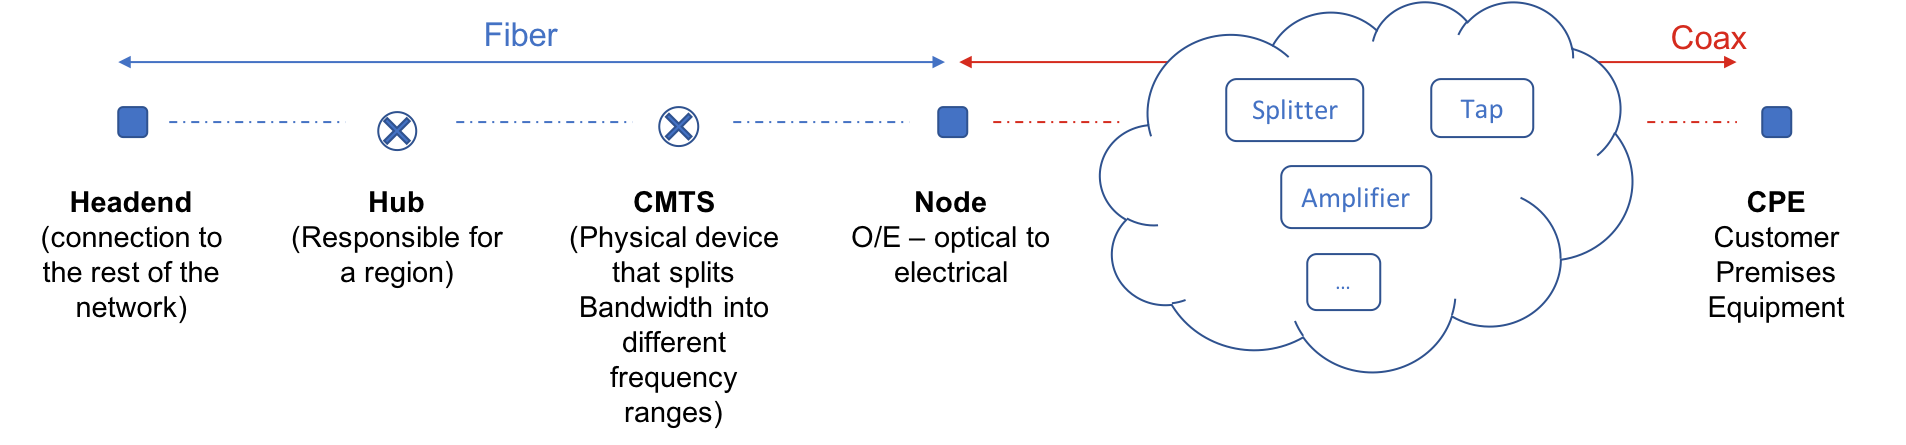
\includegraphics[width=1\linewidth]{HFC}
    \end{center}
    \caption{Hybrid Fiber-Coaxial Topology of the network}
    \label{HFC}
\end{figure}

Figure~\ref{HFC}, illustrates how a CPE is connected to the rest of the network. The only two types of device that are considered active and therefore polled by UPC frequently: CPE and CMTS. 

\begin{figure}[ht]
    \begin{center}
    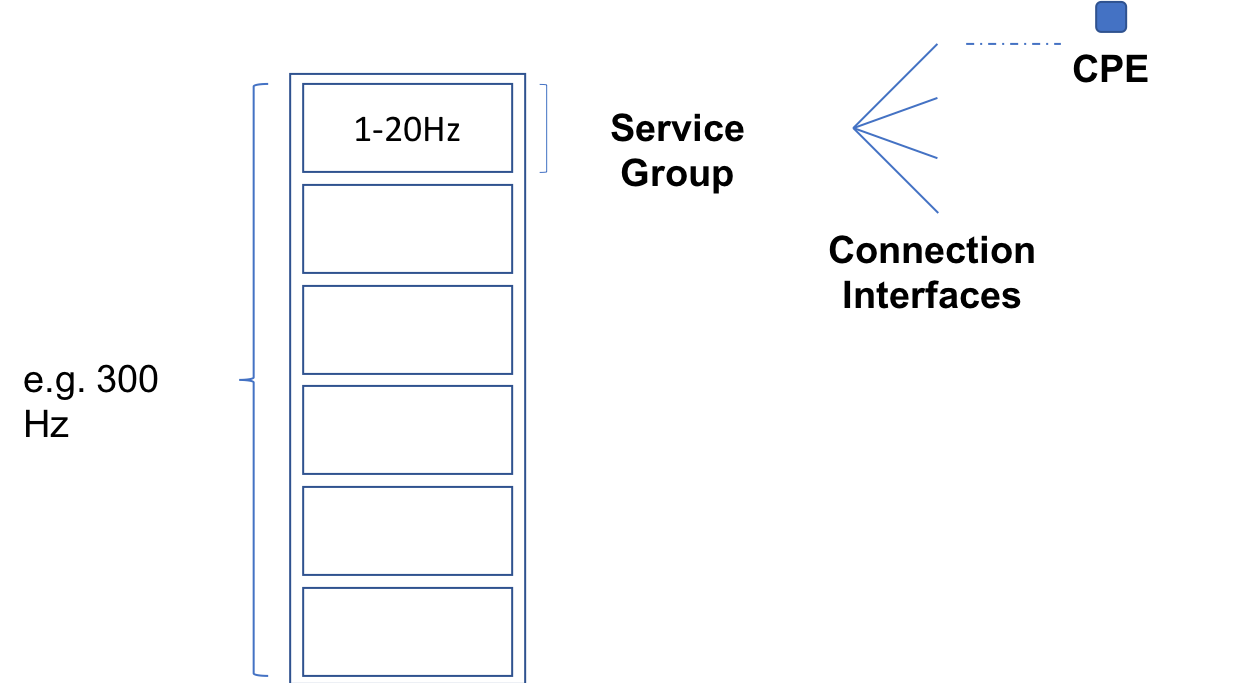
\includegraphics[width=0.5\linewidth]{SVG}
    \end{center}
    \caption{Details of the CMTS decomposition}
    \label{SVG}
\end{figure}

The CMTS \footnote{Cable Modem Termination System} splits the bandwidth into multiple frequency ranges that are called service groups, that themselves contain multiple connection interfaces (as it can be observed in Figure~\ref{SVG}. Each CPE connects to a connection interface. The connection interface that it is connected with depends on many parameters (e.g. the load of a particular interface) and changes dynamically. These dynamic changes made the mapping between a particular MAC and an interface particularly tricky to build as it is time dependent. 

\section{Data Sources}
\label{subsec:data-source} 
Because we wish to use machine learning techniques in this task in order to predict CPE failures, we need to build for each CPE a vector that will characterise it. In order to populate this vector we used different data sources that are used for multiple business needs:
\begin{itemize}
    \item SAA: UPC polls both the CMTS interfaces and CPEs every 15 minutes. Nevertheless, it isn't possible to keep all this history, therefore those measurements are aggregated hourly and kept for 11 days (10 full past days plus the current day). We will later see what measurements are monitored in such polls. 
    \item Modemloss: a Modemloss event is created whenever more than 10 CPEs go offline at the same time, then the event is logged in a database (along with its start and end date and the offline duration).
    \item VIA: whenever a customer calls the customer care service, a Session is created and the software that is used by the agent to handle the customer request will automatically keep logs of this interaction. We wish to use this database to identify failing CPEs.
\end{itemize}


\chapter{CPE Feature Vector Construction}
As opposed to data sets that are usually used in university to do Machine Learning, in the professional world those are much less frequently available and need to be built on the spot for each specific task. Therefore the first 7 weeks of the projects were entirely dedicated to data collection. 

The process was very iterative, first of all it was hard to cope with the lack of proper documentation of such databases. It was necessary to discuss with multiple persons in order to get an overview of what is available and how to interpret different data sources. But also it wasn't rare that we had to let go of the idea to use a given data source because after an initial analysis we realized that it was unusable as we will later explain for reproducibility.

In order to be as complete as necessary, we shall first discuss what measurement we decided to use to characterize a CPE and then how we decided to illustrate the time dimension of such measurements.

\section{CPE Health Indicators}
\subsection{Indicators to use}
Choosing correct measurements to monitor the health of CPEs required the collaboration with a domain expert. Namely the manager of HFC Support. His role in the company allows him to be very familiar with measurements from SAA: their range, linkage with possible issues and where those are physically collected. Table~\ref{CPEMes} presents the result of such discussion for measurements that were taken from a CPE level data source \texttt{SAA.CM\_HOUR\_HEALTH}.

\begin{table}[h]
\begin{center}
\begin{tabular}{c p{85mm}}
\hline
\textbf{Feature} & \textbf{Description}\\ 
\hline\hline
\textit{CPE's MAC address} & Allow us to uniquely identify the CPE  \\
\hline
\textit{Hardware Model} & According to domain experts, measurements can vary depending on the type of hardware (e.g. some device may have a higher mean SNR than another). \\
\hline
\textit{Service Group} & A unique identifier of the service group the CPE is connected to. It corresponds to the physical grouping of CPEs. It will help us standardize measurements among CPEs that share the same physical connections. If a problem is experienced down the topology by an element it may affect the measurement of many CPEs in the service group without causing a problem for the customer.\\
\hline
\textit{Day\textsubscript{0}} & Mostly to allow sanity checks later on (we might be interested on the date at which we start collecting data as we could observe seasonality of measurements).\\
\hline
\textit{Number of CPE in the building} & Noone knew whether or not this could affect CPE level performance and the HFC support expert advised us to drop this feature but we decided that having too much could not hurt as a first approach, which could later be droped.\\
\hline
\textit{Unavailability Percentage} & Gives an estimate of how often the CPE was offline over a given period.\\
\hline
\textit{TX Power UP} & The average upstream transmitting power.\\
\hline
\textit{RX Power UP} & The average upstream receiving power.\\
\hline
\textit{RX Power DN} & The average downstream receiving power.\\
\hline
\textit{CER DN} & Maximum codeword error downstream.\\
\hline
\textit{CER UP} & Maximum codeword error upstream.\\
\hline
\textit{SNR UP} & Sound to noise ratio upstream.\\
\hline
\textit{Percent Traffic DMH UP} & Percentage of upstream traffic computed as degraded modem hours.\\
\hline
\textit{Percent Traffic SDMH UP} & Percentage of upstream traffic computed as severally degraded modem hours.
\end{tabular}
\end{center}
\caption{\label{CPEMes}Features at the CPE level}
\end{table}

But we also needed to get information regarding the CMTS to which the CPE is connected as any problem at the CMTS can affect all nodes down the topology. For such measurement we have decided to present them in a single table regardless of the direction concerned, but an attentive reader should bear in mind that all features presented in Table~\ref{CMTSMes} are computed for upstream and downstream. 

\begin{table}[h]
\begin{center}
\begin{tabular}{c p{85mm}}
\hline
\textbf{Feature} & \textbf{Description}\\ 
\hline\hline
\textit{CMTS Name} & Part of the unique identifier of the interface\\
\hline
\textit{CMTS Interface name} & Completes the CMTS to uniquely identify the interface\\
\hline
\textit{RX Power} & Average receiving power of the CMTS\\
\hline
\textit{SNR} & Average sound to noise ratio\\
\hline
\textit{CCER} & Maximum corrected codeword error ratio\\
\hline
\textit{CER} & Maximum codeword error ratio\\
\hline
\textit{Utilization} & Average maximum percent utilization\\
\end{tabular}
\end{center}
\caption{\label{CMTSMes}Features at the CMTS level (those are collected per interface and then aggregated at the service group level)}
\end{table}

\subsection{Challenges foreseen}
During the phase of the project, we already envisioned some possible issues. We decided to list them at this stage of the report in order to address the fact that they were already identified. As a general rule, we decided that we should not address too many of them in advance as it would be possible that depending on which learning method we decide to use they could no be so problematic after all. Also it wasn't critical that we address them at such an early stage as it is essential in Machine Learning to have a baseline to which we can compare more advanced models (where advanced could mean a more complex data preparation protocol).

\begin{itemize}
    \item Aggregating so much data: the company doesn't have any spark cluster setup or any other tool that would allow the aggregation of so much data. We had the choice between setting up such cluster or to go around the problem. This solution was chosen in order to focus my work on research and not too much on such problems. Therefore it was decided that the data should be aggregated at the database level. While this required some P/L SQL it saved us a lot of setup time. 
    \item Seasonality of the data: telecommunication could be considered as an amenity in the sense that the load on the network can fluctuate heavily depending on time. And this can show at different levels: over the day, the week but also the year (e.g. different seasons means different temperature which can modify the behaviour of some component of the network). Hopefully as we will see in the following section it was possible to go around some of this seasonality.
    \item Lack of positive dataset: while VIA allow us to build a dataset of "unhealthy" CPEs thanks to customer interactions, it isn't so trivial to build a positive dataset for "healthy" CPEs. It is very probable that a customer has been experiencing problems but hasn't called customer care. This is why, before any prediction can be attempted we need to perform some clustering of the data to create a usable dataset. 
\end{itemize}

\section{Time Dimension}
As it was already mentioned numerous times in previous paragraphs, most of the indicators at the CPE and CMTS level are time dependent. Therefore we needed some way to illustrate this time dimension in our vectors. 

We define Day\textsubscript{0} as the last day at which we collect the data and assume that we have all the necessary measurements for this date up to midnight between Day\textsubscript{0} and Day\textsubscript{1}.

As an initial approach and after some discussion with the Business Intelligence team, we decided on how we could use our 10 days of history available in VIA. Two scope were defined.

\subsection{Last 24 hours}
On Day\textsubscript{0}, we consider a finer granularity as we assumed that most customer would call as soon as they experience problems with their CPEs. While we would have wanted to use the finest granularity available (1h), the HFC support manager advised us otherwise as some measurement may "flap" for no particular reason and without causing any problem. Therefore we decided to consider the average over 6 hours windowsn in order to average out such flaps.

\subsection{Last 6 days}
Then we also decided to keep daily averages from Day\textsubscript{0} to Day\textsubscript{-5} in order to see the evolution on a longer period of time. This was a trade off between the level of granularity and the number of days that could be considered. This decision was taken arbitrarily but with the idea that the team performing reporting on customer care consider a customer interaction to be a FTR\footnote{First time resolution} if the customer doesn't call back in the following 7 days, which means that most customer tend to call for problems before a period of 7 days.

\subsection{Working with relative data}
According to the HFC support expert, we are mostly interested at the evolution of indicators rather than their absolute value which is why we decided to always use relative values. We always consider an indicator as the difference between the current and the past time period. 

\section{Unusable sources}
In this section we discuss important features that were considered but could not be used as the data proved that we were wrong considering it in the first place.

\subsection{Modemloss unavailability}
Initially, it was considered essential to obtain the offline time of each CPE as it presented a very insightful information regarding its health. A first data source that was considered was the Modemloss database. As explained in Subsection~\ref{subsec:data-source}, it logs all events that cause an unavailability of more than 10 CPEs at the same time. 

One of the first problem that was experienced is that an entry in such a table consist in the identifier of the event, the mac concerned by the event, a start time, end time and offline duration. Unfortunately, the offline duration is not necessarily equal to the event length. And that can cause a serious problem to unavailability percentage computation. As we tried to illustrate it in Figure~\ref{modemloss}, we do not know from where to where a particular CPE disconnect from the network. Therefore to compute over a given time window the proportion of time during which it was unavailable cannot be done with precision. 

\begin{figure}[ht]
    \begin{center}
    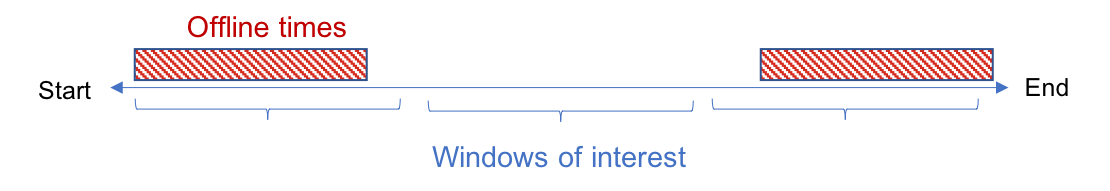
\includegraphics[width=0.7\linewidth]{images/modemloss.png}
    \end{center}
    \caption{Modemloss un-even repartition of offline times}
    \label{modemloss}
\end{figure}

Nevertheless, the product owner for this data source mentionned that such a phenomenon ($\text{offline duration} \neq \text{end} - \text{start}$) should not happen more than 2 to 3\% of the time. And that we could therefore assume the offline time to be equally distributed over the given time period. We could have indeed computed how often this happens but a second problem, more severe, appeared. Because a modemloss event is fairly rare, it would happen for a particular CPE approximately once a year and therefore would not be particularly useful with our 5 days vector representation.

In order to fight such problem we considered multiple approaches. That will also be discussed in this session as none was successful.

\subsection{SAA status flags}
SAA also contains for CPE measurement (every hour) a status indicator that tells us whether the CPE is online or not. First of all, the problem with such indicator is that it doesn't give us per say an offline period but simply an indication at a particular time (ponctual indicator) but it was decided that it could be used as a proper estimate of the offline time.

It is important to note as well that we do not have any information duplication as we monitor aggregates of our measurement. Therefore, we see a Null value for a given measurement only if all the hourly measurements come missing).
